% mnras_template.tex
%
% LaTeX template for creating an MNRAS paper
%
% v3.0 released 14 May 2015
% (version numbers match those of mnras.cls)
%
% Copyright (C) Royal Astronomical Society 2015
% Authors:
% Keith T. Smith (Royal Astronomical Society)

% Change log
%
% v3.0 May 2015
%    Renamed to match the new package name
%    Version number matches mnras.cls
%    A few minor tweaks to wording
% v1.0 September 2013
%    Beta testing only - never publicly released
%    First version: a simple (ish) template for creating an MNRAS paper

%%%%%%%%%%%%%%%%%%%%%%%%%%%%%%%%%%%%%%%%%%%%%%%%%%
% Basic setup. Most papers should leave these options alone.
\documentclass[a4paper,fleqn,usenatbib]{mnras}

% MNRAS is set in Times font. If you don't have this installed (most LaTeX
% installations will be fine) or prefer the old Computer Modern fonts, comment
% out the following line
\usepackage{newtxtext,newtxmath}
% Depending on your LaTeX fonts installation, you might get better results with one of these:
%\usepackage{mathptmx}
%\usepackage{txfonts}

% Use vector fonts, so it zooms properly in on-screen viewing software
% Don't change these lines unless you know what you are doing
\usepackage[T1]{fontenc}
\usepackage{ae,aecompl}



\usepackage{graphicx}	% Including figure files
\usepackage{amsmath}	% Advanced maths commands
\usepackage{amssymb}	% Extra maths symbols


%%%%%%%%%%%%%%%%%%% TITLE PAGE %%%%%%%%%%%%%%%%%%%

% Title of the paper, and the short title which is used in the headers.
% Keep the title short and informative.
\title[Short title, max. 45 characters]{Mg Depleted and K Enriched Stars from LAMOST Spectral Data}

% The list of authors, and the short list which is used in the headers.
% If you need two or more lines of authors, add an extra line using \newauthor
\author[Kemp et al.]{
Alex J. Kemp,$^{1}$\thanks{E-mail: ajkem1@student.monash.edu}
A. N. Other,$^{2}$
Third Author$^{2,3}$
and Fourth Author$^{3}$
\\
% List of institutions
$^{1}$Royal Astronomical Society, Burlington House, Piccadilly, London W1J 0BQ, UK\\
$^{2}$Department, Institution, Street Address, City Postal Code, Country\\
$^{3}$Another Department, Different Institution, Street Address, City Postal Code, Country
}

% These dates will be filled out by the publisher
\date{Accepted XXX. Received YYY; in original form ZZZ}

% Enter the current year, for the copyright statements etc.
\pubyear{2015}


\begin{document}
\label{firstpage}
\pagerange{\pageref{firstpage}--\pageref{lastpage}}
\maketitle

% Abstract of the paper
\begin{abstract}

\end{abstract}

% Select between one and six entries from the list of approved keywords.
% Don't make up new ones.
\begin{keywords}
keyword1 -- keyword2 -- keyword3
\end{keywords}

%%%%%%%%%%%%%%%%%%%%%%%%%%%%%%%%%%%%%%%%%%%%%%%%%%

%%%%%%%%%%%%%%%%% BODY OF PAPER %%%%%%%%%%%%%%%%%%

\section{Introduction}

This is a simple template for authors to write new MNRAS papers.
See \texttt{mnras\_sample.tex} for a more complex example, and \texttt{mnras\_guide.tex}
for a full user guide.

All papers should start with an Introduction section, which sets the work
in context, cites relevant earlier studies in the field by \citet{Others2013},
and describes the problem the authors aim to solve \citep[e.g.][]{Author2012}.

\section{Methods, Observations, Simulations etc.}

\textit{The Cannon}, a data based spectral model devloped by \cite{ho2017}, was fitted to each star in the spectra based around each star's $T_{eff}$, log(g), [Fe/H] and [$\alpha$/M].
%Ho2017 says that using Appogee, they found almost 10000 giants which were common between the lamost and apoggeee surveys and used that to fit a predictive model to the lamost giants (450000) to determine the 'Teff, logg, [Fe/H], and [α/M]'.
This model is treated as representative of the expected spectra for each star.

The residuals were taken of the normalised LAMOST flux data and 
\textit{The Cannon} according to $residual=data-model$. A positive residual implies a higher normalised flux than expected by the model, while a negative residual implies a lower normalised flux than expected. In turn, at a given spectral line a lower normalised flux is associated with an over-abundance, while a higher normalised flux is associated with a depleted abundance.

A Gaussian curve was fitted to the residuals about each spectral line in the Mg triplet (5167 \AA, 5172 \AA, 5184 \AA) as well as the K doublet (7665 \AA, 7699 \AA) to characterise any deviation from the model. The amplitude and amplitude error for this curve was then used as the basis for a data filter designed to produce potential candidate stars with spectra indicative of Mg depletion, as well as K enrichment.

Two filters were applied separately, with the candidate pool formed from all unique stars identified in either filter. The first, broader filter required the Mg 5184 line's Gaussian to satisfy $Amp > 0.05$ and $\frac{Amp}{Amp_{err}}>3$, and the K 7665 line to satisfy $Amp < 0.05$ and $\frac{Amp}{Amp_{err}}>3$. The second, more demanding filter was applied to require 2 of the three Mg lines to satisfy $Amp > 0.05$ and $\frac{Amp}{Amp_{err}}>3$, as well as either of the K lines. These filters together produced 280 candidate stars to be vetted manually.

The vetting process was done through visual examination of each case. The minimum criterion for a pass was two out of the three Mg lines to look at least plausibly depleted, and at least one of the K lines to look convincing. The local noisiness of the signal was taken into account when making these determinations. Of the 280 candidates manually vetted, 156 were ultimately determined to be sufficiently strong candidates to make the list, presented in Table [INSERT TABLE REFERENCE HERE].

\subsection{Figures and tables}

Figures and tables should be placed at logical positions in the text. Don't
worry about the exact layout, which will be handled by the publishers.

Figures are referred to as e.g. Fig.~\ref{fig:example_figure}, and tables as
e.g. Table~\ref{tab:example_table}.


\begin{figure}
	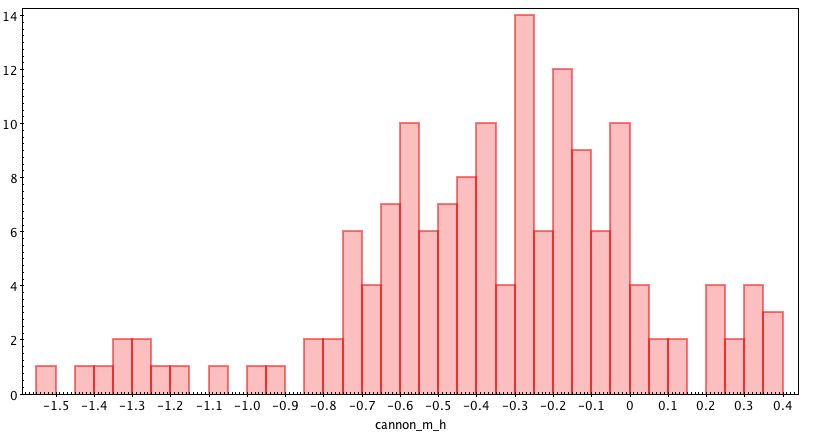
\includegraphics[width=\columnwidth]{m_hhist.png}
    \caption{Metalicity Histogram}
    \label{mhist}
\end{figure}

\begin{figure}
	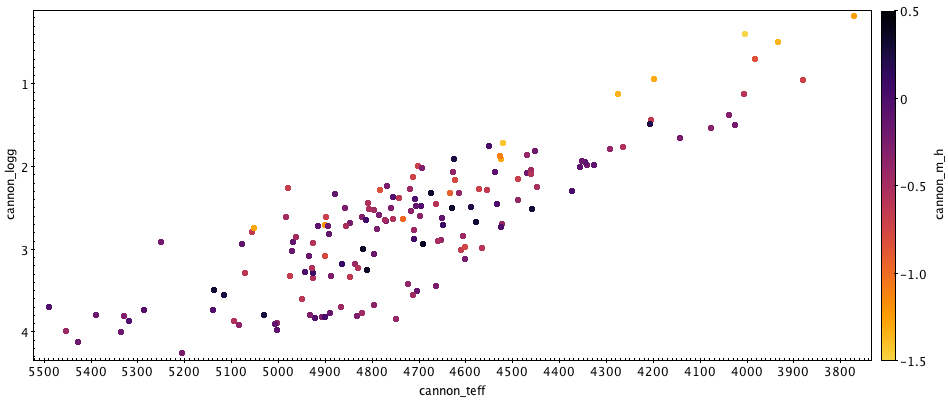
\includegraphics[width=\columnwidth]{teff_logg.png}
    \caption{Effective temperature, log surface gravity, metalicity}
    \label{mhist}
\end{figure}

\begin{figure}
	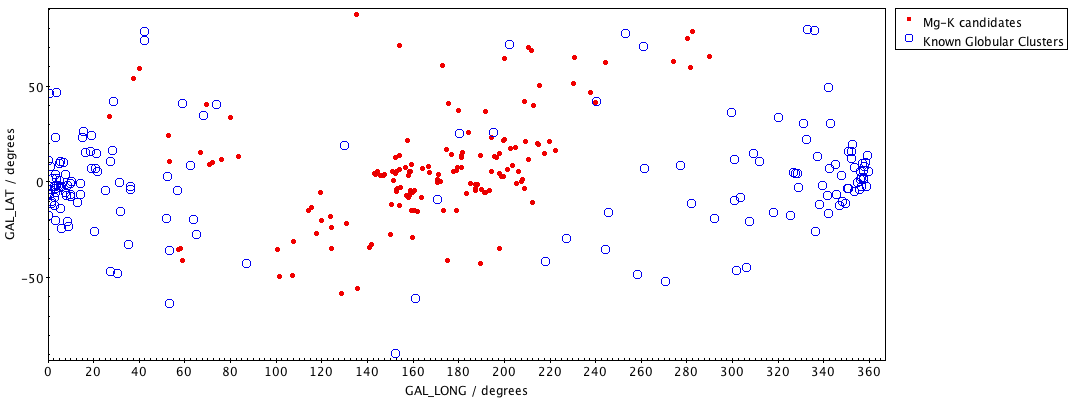
\includegraphics[width=\columnwidth]{galcoord.png}
    \caption{Galactic coordinates for Mg-K stars and known globular clusters}
    \label{mhist}
\end{figure}

% Example table
\begin{table}
	\centering
	\caption{This is an example table. Captions appear above each table.
	Remember to define the quantities, symbols and units used.}
	\label{tab:example_table}
	\begin{tabular}{lccr} % four columns, alignment for each
		\hline
		A & B & C & D\\
		\hline
		1 & 2 & 3 & 4\\
		2 & 4 & 6 & 8\\
		3 & 5 & 7 & 9\\
		\hline
	\end{tabular}
\end{table}


\section{Conclusions}

The last numbered section should briefly summarise what has been done, and describe
the final conclusions which the authors draw from their work.

\section*{Acknowledgements}

The Acknowledgements section is not numbered. Here you can thank helpful
colleagues, acknowledge funding agencies, telescopes and facilities used etc.
Try to keep it short.

%%%%%%%%%%%%%%%%%%%%%%%%%%%%%%%%%%%%%%%%%%%%%%%%%%

%%%%%%%%%%%%%%%%%%%% REFERENCES %%%%%%%%%%%%%%%%%%

% The best way to enter references is to use BibTeX:

\bibliographystyle{mnras}
\bibliography{mgkbib} % if your bibtex file is called example.bib


% Alternatively you could enter them by hand, like this:
% This method is tedious and prone to error if you have lots of references


%%%%%%%%%%%%%%%%%%%%%%%%%%%%%%%%%%%%%%%%%%%%%%%%%%

%%%%%%%%%%%%%%%%% APPENDICES %%%%%%%%%%%%%%%%%%%%%

\appendix

\section{Some extra material}

If you want to present additional material which would interrupt the flow of the main paper,
it can be placed in an Appendix which appears after the list of references.

%%%%%%%%%%%%%%%%%%%%%%%%%%%%%%%%%%%%%%%%%%%%%%%%%%


% Don't change these lines
\bsp	% typesetting comment
\label{lastpage}
\end{document}

% End of mnras_template.tex